\documentclass{article} % For LaTeX2e
\usepackage{nips11submit_e,times}
\usepackage[lined,boxed,commentsnumbered]{algorithm2e}
\usepackage{amsmath}
%\documentstyle[nips10submit_09,times,art10]{article} % For LaTeX 2.09


\title{Predicting the Tags of Questions in StackOverflow}

\newcommand{\fix}{\marginpar{FIX}}
\newcommand{\new}{\marginpar{NEW}}

%\nipsfinalcopy % Uncomment for camera-ready version

\begin{document}

\maketitle

\begin{abstract}
Under construction
\end{abstract}

\section{Introduction}

As the world's most popular programmer Q\&A community, StackOverflow.com is a showcase of the successful usage of the tagging system, where each question could have one or more tags to indicate its ``topics". 

Traditional hierarchical taxonomies force each item to be one of the predefined categories, however in a tagging system one item could have multiple categories(the ``tags"). Moreover, the tagging systems normally encourages users to contribute their own tags. Thus, by gathering the ``wisdom of the crowd", an item can have more up-to-date and precise descriptors.

In this project we aim at predicting the tags of a question by analyzing the tagged questions/answers from StackOverflow.com. That is, given a question, our system will predict appropriate tags for it. With the tag predictor, a user could have suggested tags at hand as soon as he/she asked a question. This will facilitate tagging task. Sen et al.\cite{Sen2006} point out that with suggestion people are more likely to assign items with higher quality tags.

Moreover, the tag prediction will also benefit the already tagged questions by giving us a deeper insight into that question in the following ways:

\begin{itemize}
    \item Reveal the hidden tags: often a piece of text is a mix of different topics while a user may only choose a fraction of them as the tags. That is to say, these tags only indicate the ``partial topics" of the text. With the tag prediction technology, we're able to discover the ``hidden" tags.
    \item Discover the Vocabulary difference: different users may use different terms to describe the same item. Our predictor can be a good assistant in finding the synonym tags because similar tag by searching tags with similar word distribution.
    \item Disambiguation: tags are short and often ambiguous. With additionally predicted tags it will easier grasp the meaning of a specific tag. For example, an article with tag ``apple" may tell us little of its content, but if we find the hidden tags ``osx", ``iphone" then we know exactly what ``apple" mean under such context.
\end{itemize}

In this project, we will adopt and improve several methods to predict the tags of the questions in StackOverflow.com. Unlike traditional classification problems, tag assignment is harder owing to its subjectivity and incompleteness. We'll discuss more about this in experiment section.


\section{Related Work}

\subsection{Tagging System}
\subsection{Text Classfication}
\subsection{Social Tag Prediction}


\section{Proposed Method}

\subsection{Naive Bayes}
Naive Bayes classifier is a simple yet powerful classifier based on Bayes theorem. It assumes that the presence of one feature is independent from the presence of the others. When performing the text categorization, Naive Bayes treats each document as a ``bag of words" and words are conditionally independent from each other.

In practice, naive Bayes classifiers can have a very satisfactory performance in a supervised learning. Many real-world problems are tackled by naive Bayes. Owing to its simplicity and desirable accuracy in many cases, we chose naive Bayes as our baseline.

By applying Bayes theorem, we can get the label $Y$'s probability given $X$.
\begin{gather}
    P(Y \vert X_1,\dots,X_n) = \frac{P(Y) \ P(X_1,\dots,X_n\vert Y)}{P(X_1,\dots,X_n)}. 
\end{gather}

With the independence assumption, the classification problem is equivalent to:
\begin{gather}
    \mathrm{y} = \underset{y}{\operatorname{argmax}} \ P(Y=y) \displaystyle\prod_{i=1}^n P(X_i=x_i\vert Y=y).
\end{gather}
The training algorithm is stated in Algorithm\ref{alg:nb}.

\IncMargin{1em}
\begin{algorithm}
\label{alg:nb}
\SetKwData{Left}{left}\SetKwData{This}{this}\SetKwData{Up}{up}
\SetKwFunction{Union}{Union}\SetKwFunction{FindCompress}{FindCompress}
\SetKwInOut{Input}{Input}\SetKwInOut{Output}{Output}
\Input{Training set $T=\{t_1,...t_n\}$}
\Output{$P(Y)$ and  $P(X|Y)$}
\BlankLine
Initialize all $Count(y)$ and $Count(x|y)$ to be 0\;
Initialize total count $N$ to be 0\;

\ForEach{$t \in T$} {
    $X_t, y_t$ = $t$\;
    \ForEach{$x \in X_t$} {
        $Count(y) \leftarrow Count(x) + 1$ \;
        $Count(x|y) \leftarrow Count(x|y) + 1$ \;
        $N \leftarrow N$ + 1 \;
    }
}
% Calculate $P(Y), P(X|Y)$ from $Count(Y), Count(X|Y)$ and $N$}
\Return $P(Y), P(X|Y) \leftarrow CalculateProbability(Count(Y), Count(X|Y), N)$

\caption{Naive Bayes Training Algorithm}\label{algo_disjdecomp}
\end{algorithm}
\DecMargin{1em}

\subsection{Logistic Regression}

Logistic regression is a discriminative model which learns $P(Y|X)$ directly from the training data. In our problem the value of $y$ takes any of the discrete values $\{y_1,...y_K\}$, and the form of $P(Y=y_k|X)$ for $Y=y_1,...Y=y_{K-1}$ is: 

\begin{gather}
	P(Y=y_k|X)=\frac{exp(w_{k0}+\sum_{i=1}^n{w_{ki}X_i})}{1+\sum_{j=1}^{K-1}exp(w_{j0}+\sum_{i=1}^n{w_{ji}X_i})}
\end{gather}

For $Y=y_K$, the form is:
\begin{gather}
	P(Y=y_K|X)=\frac{1}{1+\sum_{j=1}^{K-1}exp(w_{j0}+\sum_{i=1}^n{w_{ji}X_i})}
\end{gather}

Here $X_i$ denotes the $i$th variable in $X$, and $w_{ji}$ means the weight of $j$th class of $Y$ with variable $X_i$.

If using gradient descent rule with regularization in order to estimate the values of $w_{ji}$, we are after:
\begin{gather}
	w_{ji} \leftarrow w_{ji}+ \eta \sum_{l}X_{i}^{l}(\delta (y_{j} \in Y^{l})-\hat{P}(y_{j} \in Y^{l}|X^{l},W))- \eta \lambda w_{ji}
\end{gather}
where $\eta$ is a small constant which determines the step size, and $\lambda$ is the regularization constant. The algorithm is stated in Algorithm \ref{alg:lr}.

\IncMargin{1em}
\begin{algorithm}
\label{alg:lr}
\SetKwData{Left}{left}\SetKwData{This}{this}\SetKwData{Up}{up}
\SetKwFunction{Union}{Union}\SetKwFunction{FindCompress}{FindCompress}
\SetKwInOut{Input}{Input}\SetKwInOut{Output}{Output}
\Input{Training set $T=\{t_1,...t_n\}$, constant $\eta$, converge threshold $\varepsilon$, regulation factor $\lambda$}
\Output{Weight matrix $W$}
\BlankLine
Initialize all $w_{ji} \in W$ to 0\;
$isConverge \leftarrow false$\;
\While{$isConverge = false$}{
	\ForEach{$w_{ji} \in W$}{
		\ForEach{$t_l \in T$}{
			$jump_{ji} \leftarrow 0$\;
			Calculate $d=X_{i}^{l}(\delta (y_{j} \in Y^{l})-\hat{P}(y_{j} \in Y^{l}|X^{l},W))$\;
			$jump_{ji} \leftarrow \eta * d$\;
		}
		$w_{ji} \leftarrow w_{ji} + jump_{ji}$\;
	}
	$w_{ji} \leftarrow w_{ji} - \eta \lambda w_{ji}$\;
	\If{$\forall jump_{ji} \rightarrow jump_{ji} < \varepsilon$}{
		$isConverge \leftarrow true$\;
	}
}
\Return $W$\;
\caption{Logistic Regression Training Algorithm}\label{algo_disjdecomp}
\end{algorithm}
\DecMargin{1em}

% TODO: CURIOUS CASE OF STRANGE LAYOUT
% \pagebreak

\subsection{Neural Networks}

Neural Networks is another classifier model that can be applied to our problem. In our case, the input units represent words in the question, and output units represent tags. We add one hidden layer in this network (normally one hidden layer is enough), and use backpropagation to train the weights. 

Our algorithm for training the Neural Networks is stated in Algorithm \ref{alg:nn}. Each training sample is a vector pair $<\overrightarrow{x},\overrightarrow{y}>$, where $\overrightarrow{x}$ is the vector of network input values, and $\overrightarrow{y}$ is the target network output values. $\eta$ is a small constant set to 0.05. $n_w$, $n_h$ and $n_t$ stand for the number of words, the number of hidden units and the number of tags, respectively. $w_{wh}$ is the weight from a word unit to a hidden unit, and $w_{ht}$ is the weight from a hidden unit to a tag unit. The algorithm outputs two weight matrix consisting all the weights of $w_{wh}$ and $w_{ht}$.

\IncMargin{1em}
\begin{algorithm}
\label{alg:nn}
\SetKwData{Left}{left}\SetKwData{This}{this}\SetKwData{Up}{up}
\SetKwFunction{Union}{Union}\SetKwFunction{FindCompress}{FindCompress}
\SetKwInOut{Input}{Input}\SetKwInOut{Output}{Output}
\Input{Training set $T=\{t_1,...t_n\}$, constant $\eta$, $n_w$, $n_h$, $n_t$}
\Output{Two weight matrix $W_{wh}$ and $W_{hy}$}
\BlankLine
Create a feed-forward neural network with $n_w$ input units, $n_h$ hidden units and $n_t$ output units\;
Initialize all $w_{wh} \in W_{wh}$ and $w_{ht} \in W_{ht}$ to be small random numbers between $(-0.05, 0.05)$\;
\ForEach{Training sample $<\overrightarrow{x},\overrightarrow{y}>$}{
	Compute $O_{w}^{l}=\sigma (\overrightarrow{w}*\overrightarrow{x})$ and $O_{h}^{l}=\sigma (\overrightarrow{w}*\overrightarrow{O_{w}^{l}})$ 
		where $\sigma (y)=\frac{1}{1+exp\{-y\}}$ \;
	For each $O_{w}^{l}$, compute $\delta_{w}^{l} \leftarrow O_{w}^{l} (1-O_{w}^{l}) (t_{w}^{l} - O_{w}^{l})$ \;
	For each $O_{h}^{l}$, compute $\delta_{h}^{l} \leftarrow O_{h}^{l} (1-O_{h}^{l}) \sum_{w \in outputs}{w_i \delta_{k}^{l}}$ \;
	For each $w_{wh} \in W_{wh}$, compute $w_{wh} \leftarrow w_{wh}+\eta \delta_{w}^{l}O_{w}^{l}$ \;
	For each $w_{ht} \in W_{ht}$, compute $w_{ht} \leftarrow w_{ht}+\eta \delta_{h}^{l}O_{h}^{l}$ \;
}
\Return $W_{wh}$ and $W_{ht}$ \;

\caption{Neural Networks Training Algorithm}\label{algo_disjdecomp}
\end{algorithm}\DecMargin{1em}


\section{Experiments}
\section{Experiments}

\subsection{Dataset and Evaluation Methods}
The dataset used in our experiments is provided by StackOverflow.com. Currently, there are 2.2 million questions, 4.8 millions answers, over 35 thousands tags in this dataset\cite{DataDump}.

We prepared 1,050,000 posts (a post is either a question or an answer)  as the training data $S_{train}$. Also we randomly sampled 5 groups of test data, each with 1000 posts.$S_{test}^i, i \in [1, 5]$.

In our experiments, precision and recall are the metrics to evaluation the predicted results. Here is the definition of the \emph{precision} and \emph{recall}:
$$ \text{Precision}=\frac{tp}{tp+fp}, \text{Recall}=\frac{tp}{tp+fn} $$
where $tp$ is the number of true positive samples, $fp$ is the number of false positive samples and $fn$ is the number of false negative samples.

As we mentioned in \emph{Introduction}, the big challenge of tag prediction is that tags are often quite subjective and incomplete. As a result, it will be problematic to conclude that a tag is "correctly" predicted only when it appears in user-defined tags. For example, if a question is tagged with "java" but predicted tag is "jdk", we still believe it is a \emph{"good"} prediction because in real life, "jdk" is closed related with "java".

Thus, instead of measure the "goodness" of a tag with only \emph{match/unmatch}, we assign each predicted tag with a relevance score $s, s \in [0, 1]$. The higher the score, the more
relevant two tags are.

To get the relevance score $s$, we proposed two methods:
\begin{itemize}
    \item{Kullback-Leibler divergence}: Kullback–Leibler is an asymmetric measure of the difference between two probability distributions $P$ and $Q$. In our case, each tag has a corresponding \emph{word distribution} and we assume that similar tags will often have similar word distribution.
    \item{Co-occurrence rate}: an alternative way for the similarity measurement is to calculate the co-occurrence rate between predicted tags and user-defined tags. Co-occurrence is asymmetrical and is very suitable to infer from sub-type tag to parent-type tag. For example, with co-occurrence rate, the predicted tag "jdk" is very relevant to user-defined tag "java". However, the co-occurrence rate from "java" to "jdk" will be much smaller.
\end{itemize}

These tools enable automatic test and thus ease the evaluation on large test set.

\subsection{Experimental Results}
\subsubsection{Naive Bayes}
In naive Bayes, we choose the top-rank $N$ tags as our predicted tags. Figure \ref{fig:naive} shows the precision/recall of Bayes classifier with different $N$. We can see that the recall increases as $N$ goes up; whereas the precision drops when $N$ increases.

\begin{figure}[htb!]
\centering%
    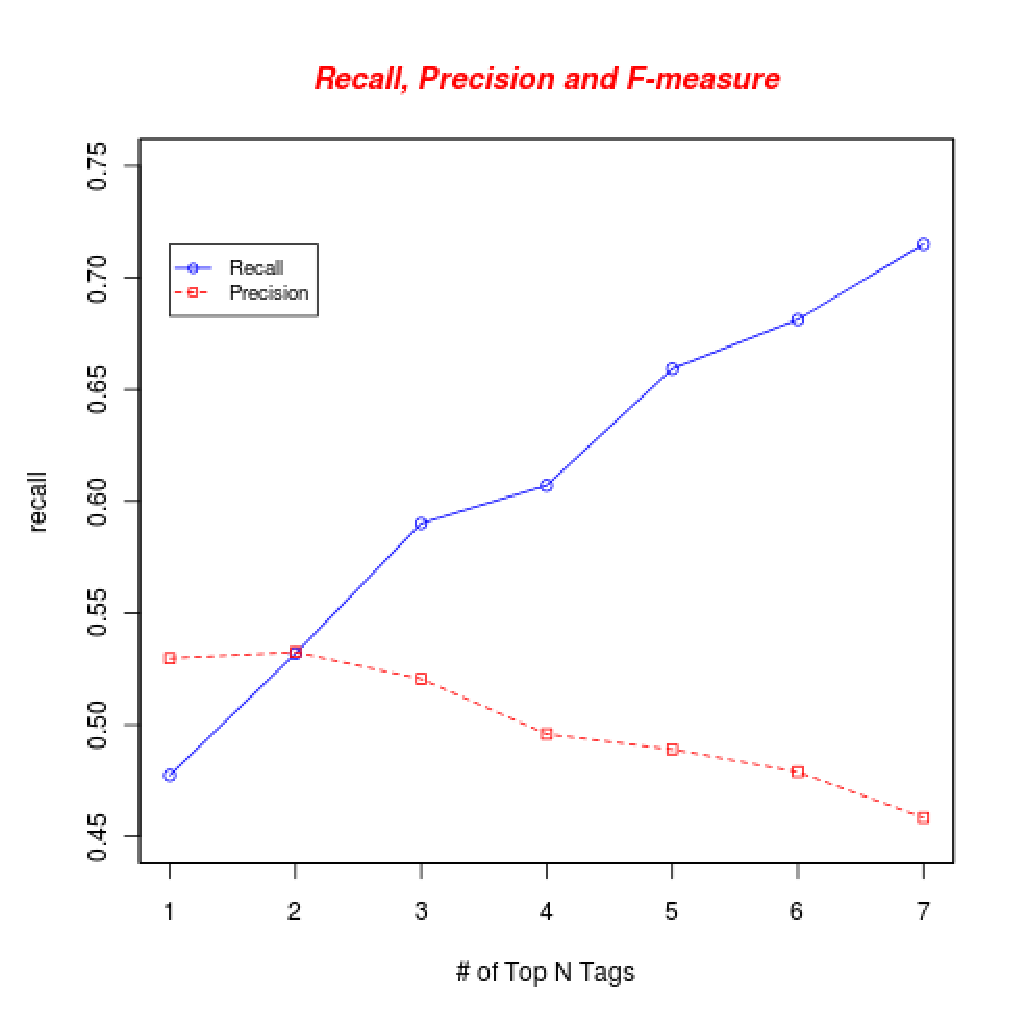
\includegraphics[scale=0.42]{naives.eps}
\caption{Tag Prediction By Naive Bayes}
\label{fig:naive}
\end{figure}

\subsubsection{Logistic Regression}
Under Construction

\subsubsection{Neural Networks}
Under Construction

\subsection{Comparison and Conclusion}
Under Construction. This part depends on the experimental results of all the three models.


\section{Reference}
\small{
\bibliography{ref}
\bibliographystyle{plain}
}

\end{document}
